\documentclass[a4paper]{article}      % The type of the document.
\usepackage{latexsym,bm,amsthm,amsmath,fancyhdr}

\usepackage[pdftex]{graphicx,xcolor}
\usepackage{epsf}
\setlength{\voffset}{-15.4mm}
\setlength{\textwidth}{150mm}
\title{The exact solution of right-angled triangular plate problem by solving functional equations}% The title and author of the document.

\begin{document}
\maketitle
\graphicspath{{Figures/}}
\section{Introduction}
The lateral deflection in plain-plate problem is described by the equilibrium equation
    \begin{equation}\label{ref:equation:1}                                       %Equation(1)
    \frac{\partial^{4}w}{\partial x^{4}}+ 2\frac{\partial^{4}w}{\partial x^{2} \partial y^{2}}+\frac{\partial^{4}w}{\partial y^{4}}=p(x,y)
    \end{equation}
where $ p(x,y)$ is a continuously distributed lateral load.
The general solution of the partial Equation (\ref{ref:equation:1}) is given by
    \begin{equation}\label{ref:equation:2}                                       %Equation(2)
    w(x,y)=w_{0}(x,y)+\varphi_{1}(x+iy)+\varphi_{2}(x-iy)+x[\psi_{1}(x+iy)+\psi_{2}(x-iy)]
    \end{equation}
where $w_{0}(x,y)$ is a particular solution of Equation (\ref{ref:equation:1}) and $\varphi_{1}$,$\varphi_{2}$,$\psi_{1}$,$\psi_{2}$ are four arbitrary functions.
The problem of a clamped right-angled triangular plate can be expressed as follow:
\begin{equation}\label{ref:equation:3}                                       %Equation(3)
     \left\{ {\begin{array}{*{20}{c}}
    {\frac{\displaystyle {{\partial ^4}w}}{\displaystyle {\partial {x^4}}} + 2\frac{\displaystyle {{\partial ^4}w}}{\displaystyle {\partial {x^2}\partial {y^2}}} + \frac{\displaystyle {{\partial ^4}w}}{\displaystyle {\partial {y^4}}} = p(x,y)}\\
    {w(x,0)=\frac{\displaystyle {\partial w}}{\displaystyle {\partial y}}(x,0)=0}\\
    {w(0,y)=\frac{\displaystyle {\partial w}}{\displaystyle {\partial x}}(0,y)=0}\\
    {w(x,y)_{l}=\frac{\displaystyle {\partial w}}{\displaystyle {\partial n}}(x,y)_{l}=0}
    \end{array}} \right.
    \end{equation}
$l$ means the hypotenuse of the triangle. $\frac{{\partial w}}{{\partial n}}$ means the directional derivative of $w$ along $\vec{n}$. $\vec{n}$ is perpendicular to $l$. The triangular plate can be shown as Figure (\ref{ref:figure:1}).
\begin{figure}
  % Requires \usepackage{graphicx}
  \centering
  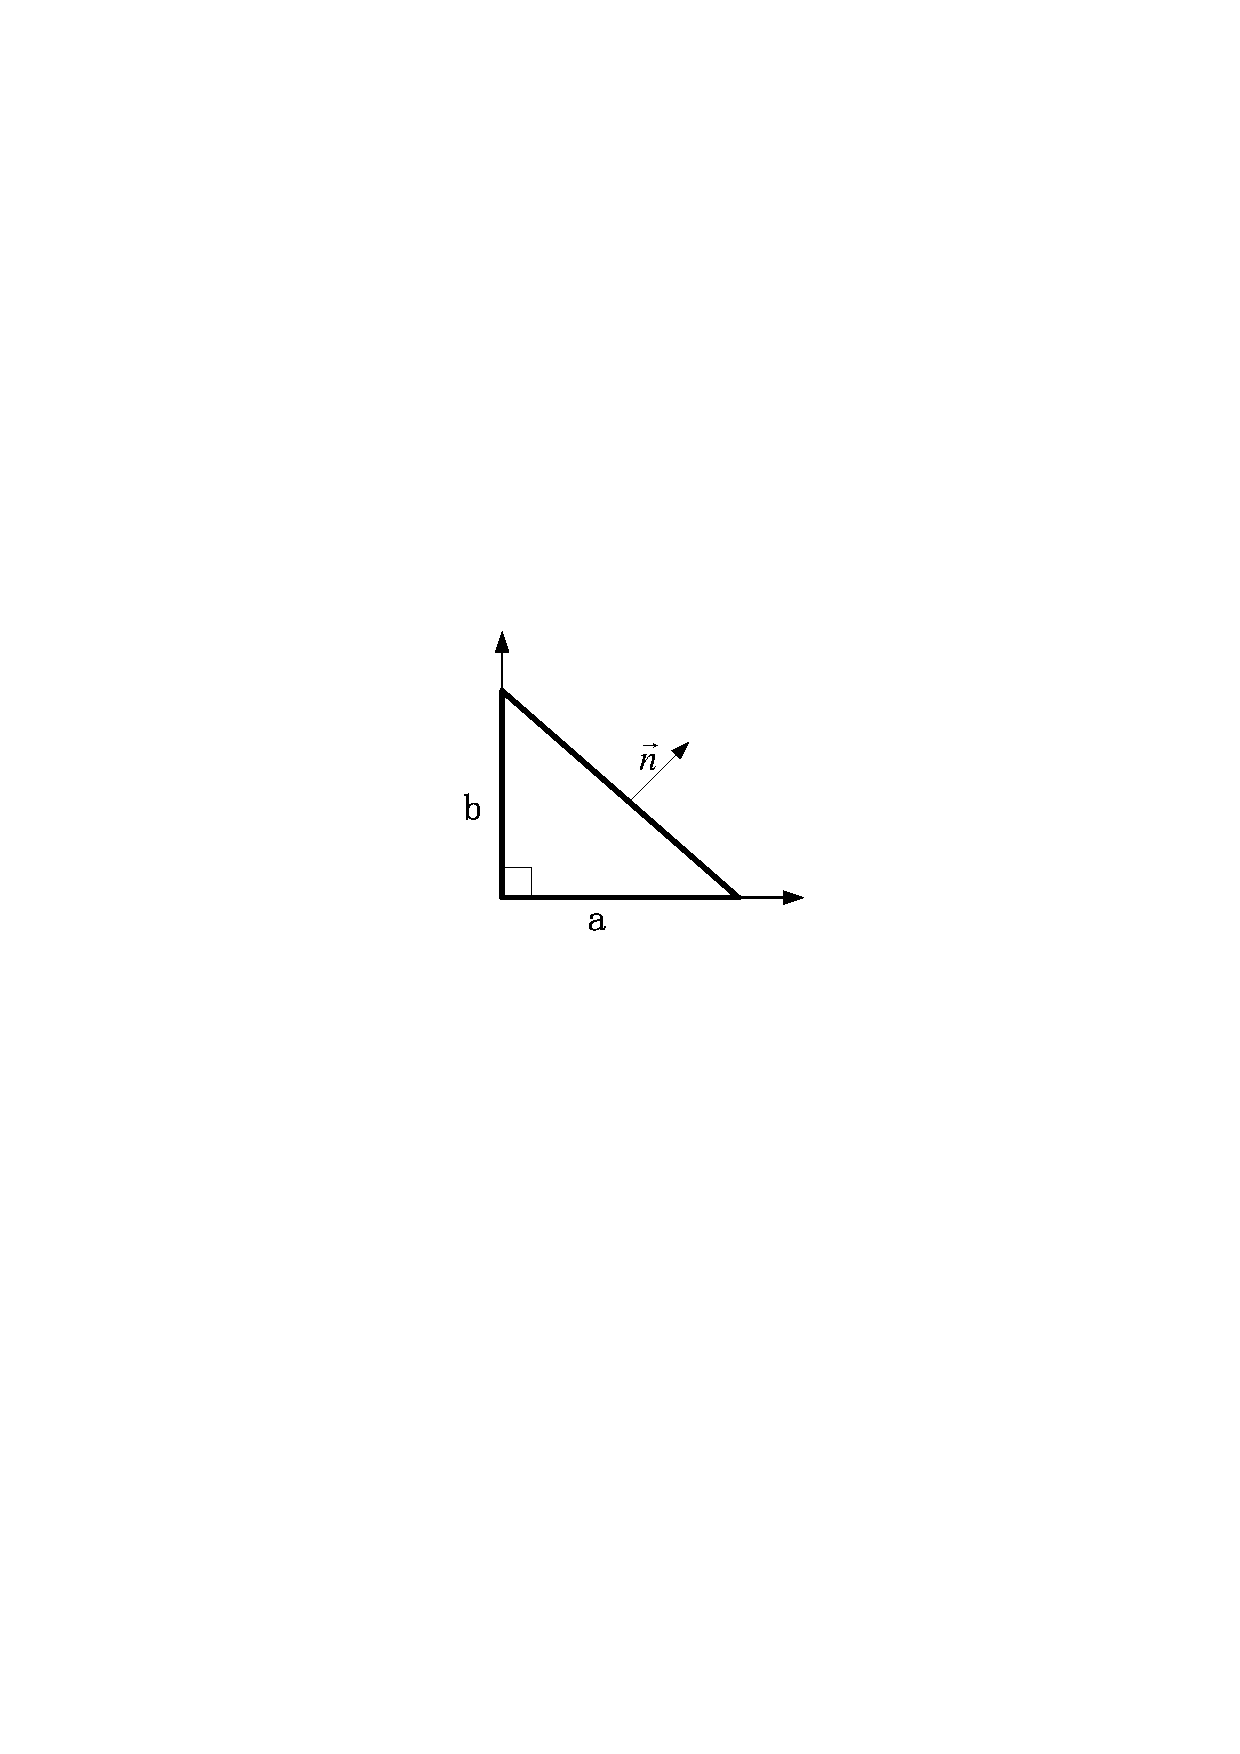
\includegraphics[width=4cm]{triangularplate.pdf}\\
  \caption{The clamped right-angled triangular plate}\label{ref:figure:1}
\end{figure}

\newtheorem{theorem}{Theorem}[section]
\begin{theorem}                                                             %This is the theorem
  (All boundaries are clamped) The solution of the equations (\textnormal{\ref{ref:equation:3}})
is given by
\end{theorem}
\begin{proof}[{\bf Proof}]%
\item[\quad Step 1.] To make the solution (\ref{ref:equation:2}) satisfies the boundary conditions $w(x,0)=0$ and $\frac{\partial w}{\partial y}(x,0)=0$, we must put
         \begin{equation}\label{ref:equation:4}                                 %Equation(4)
         \begin{split}
         \varphi_{1}(x)+\varphi_{2}(x)+x[\psi_{1}(x)+\psi_{2}(x)]&=A(x)\\
         \varphi_{1}'(x)-\varphi_{2}'(x)+x[\psi_{1}'(x)-\psi_{2}'(x)]&=B(x)\\
         \end{split}
         \end{equation}
    where $A(x)=-w_{0}(x,0)$ and $B(x)=i\frac{\displaystyle \partial w_{0}}{\displaystyle \partial y}(x,0)$. Letting
         \begin{equation}\label{ref:equation:5}                                 %Equation(5)
           \varphi_{1}(x)+x\psi_{1}(x)=\alpha(x)
         \end{equation}
    where $\alpha(x)$ is an arbitrary function. By (\ref{ref:equation:5}) and the first equation of Eqs.(\ref{ref:equation:4}), we have
         \begin{equation}\label{ref:equation:6}                                 %Equation(6)
          \varphi_{2}(x)+x\psi_{2}(x)=A(x)-\alpha(x)
         \end{equation}
    (\ref{ref:equation:5}) and (\ref{ref:equation:6}) imply that
         \begin{equation}\label{ref:equation:7}                                 %Equation(7)
         \left\{ {\begin{array}{*{20}{l}}
         {\varphi_{1}(x)=-x\psi_{1}(x)+\alpha(x)}\\
         {\varphi_{2}(x)=-x\psi_{2}(x)+A(x)-\alpha(x)}
         \end{array}} \right.
         \end{equation}
    Substituting (\ref{ref:equation:7}) into the second equation of Eqs. (\ref{ref:equation:4}) yields
        \begin{equation}\label{ref:equation:8}                                  %Equation(8)
        \psi_{2}(x)=\psi_{1}(x)-2\alpha'(x)+A_{1}(x)
        \end{equation}
    where $A_{1}(x)=A'(x)+B(x)$. By (\ref{ref:equation:7}) and (\ref{ref:equation:8}), we get
        \begin{equation}\label{ref:equation:9}                                  %Equation(9)
        \left\{ {\begin{array}{*{20}{l}}
         {\varphi_{1}(x)=-x\psi_{1}(x)+\alpha(x)}\\
         {\varphi_{2}(x)=-x\psi_{1}(x)+2x\alpha'(x)-\alpha(x)+A_{2}(x)}\\
         {\psi_{2}(x)=\psi_{1}(x)-2\alpha'(x)+A_{1}(x)}
        \end{array}} \right.
        \end{equation}
    where $A_{2}(x)=A(x)-xA_{1}(x)$.%

    Then the solution can be expressed as
    \begin{equation}\label{ref:equation:10}
    w(x,y)={w_1}(x,y) - iy\psi_{1}(x + iy) + iy\psi_{1}(x - iy) + \alpha (x + iy) - \alpha (x - iy) - 2iy\alpha '(x - iy)
    \end{equation}
    where ${w_1}(x,y) = {w_0}(x,y) + {A_2}(x - iy) + x{A_1}(x - iy)$.
\item[\quad Step 2.]Similarly, to make the solution (\ref{ref:equation:2}) satisfies the boundary conditions $w(0,y)=0$ and $\frac{{\partial w}}{{\partial x}}(0,y)=0$, we must put
    \begin{equation}\label{ref:equation:11}
    \left\{ {\begin{array}{*{20}{l}}
    {-iy\psi_{1}(iy)+iy\psi_{1}(-iy)+\alpha(iy)-\alpha(-iy)-2iy\alpha'(-iy)=C(y)}\\
    {-iy\psi_{1}'(iy)+iy\psi_{1}'(-iy)+\alpha'(iy)-\alpha'(-iy)-2iy\alpha''(-iy)=D(y)}
    \end{array}}\right.
    \end{equation}

where $C(y)=-w_1(0,y)$, $D(y)=-\frac{\displaystyle \partial w_1}{\displaystyle \partial x}(0,y)$.

Now, we differentiate the first equation of Eqs.(\ref{ref:equation:11}) with respect to $y$, then we get
    \begin{equation}\label{ref:equation:12}
    -i\psi_1(iy)+i\psi_{1}(-iy)+y\psi_{1}'(iy)+y\psi_{1}'(-iy)+i\alpha'(iy)-i\alpha'(-iy)-2y\alpha''(-iy)=C'(y)
    \end{equation}

It is easy to rewrite the first equation of Eqs.(\ref{ref:equation:11}) as follow:
\begin{equation}\label{ref:equation:13}
\psi_{1}(iy)-\psi_{1}(-iy)=\frac{\alpha(iy)-\alpha(-iy)}{iy}-2\alpha'(-iy)-\frac{C(y)}{iy}
\end{equation}

Substituting equation(\ref{ref:equation:13}) to equation(\ref{ref:equation:12}) yields
\begin{equation}\label{ref:equation:14}
-\frac{\alpha(iy)-\alpha(-iy)}{y}+i\alpha'(iy)+i\alpha'(-iy)-2y\alpha''(-iy)+y\psi_{1}'(iy)+y\psi_{1}'(-iy)=-\frac{C(y)}{y}+C'(y)
\end{equation}

By the second equation of Eqs.(\ref{ref:equation:11}) and equation(\ref{ref:equation:14}), we can get
\begin{equation}\label{ref:equation:15}
y\psi_{1}'(iy)-y\psi_{1}'(-iy)=-i\alpha'(iy)+i\alpha'(-iy)-2y\alpha''(-iy)+iD(y)
\end{equation}
\begin{equation}\label{ref:equation:16}
y\psi_{1}'(iy)+y\psi_{1}'(-iy)=\frac{\alpha(iy)-\alpha(-iy)}{y}-i\alpha'(iy)-i\alpha'(-iy)+2y\alpha''(-iy)-\frac{C(y)}{y}+C'(y)
\end{equation}

By (\ref{ref:equation:16})+(\ref{ref:equation:15}), we obtain
\begin{equation}\label{ref:equation:17}
2y\psi_{1}'(iy)=\frac{\alpha(iy)-\alpha(-iy)}{y}-2i\alpha'(iy)+iD(y)-\frac{C(y)}{y}+C'(y)
\end{equation}

By (\ref{ref:equation:16})$-$(\ref{ref:equation:15}), we obtain
\begin{equation}\label{ref:equation:18}
2y\psi_{1}'(-iy)=\frac{\alpha(iy)-\alpha(-iy)}{y}-2i\alpha'(-iy)+4y\alpha''(-iy)-iD(y)-\frac{C(y)}{y}+C'(y)
\end{equation}

Let $y\rightarrow -y$ in equation(\ref{ref:equation:18}), we have
\begin{equation}\label{ref:equation:19}
-2y\psi_{1}'(iy)=\frac{\alpha(-iy)-\alpha(iy)}{-y}-2i\alpha'(iy)-4y\alpha''(iy)-iD(-y)-\frac{C(-y)}{-y}+C'(-y)
\end{equation}

By (\ref{ref:equation:17})+(\ref{ref:equation:19}), we obtain
\begin{equation}\label{ref:equation:20}
2\frac{\alpha(iy)-\alpha(-iy)}{y}-4i\alpha'(iy)-4y\alpha''(iy)+iD(y)-iD(-y)-\frac{C(y)}{y}+\frac{C(-y)}{y}+C'(y)+C'(-y)=0
\end{equation}

Simplify equation(\ref{ref:equation:20}), we get
\begin{equation}\label{ref:equation:21}
2\alpha(iy)-2\alpha(-iy)-4iy\alpha'(iy)-4y^2\alpha''(iy)+iyD(y)-iyD(-y)-C(y)+C(-y)+yC'(y)+yC'(-y)=0
\end{equation}
\end{proof}
%-------------Solving equation 21
\newtheorem{lemma}[theorem]{Lemma}
\begin{lemma}\label{lemma 1}
    The general solution of the function equation(\textnormal{\ref{ref:equation:21}}) can be written as
    \begin{equation}\label{ref:equation:22}                                     %Equation(25)
    \alpha(x)=\alpha_0(x)+\sum_{n=1}^{\infty}a_n x^{\lambda_n}
    \end{equation}
where
    \begin{equation}\label{ref:equation:23}                                     %Equation(25)
    2\lambda^2-4\lambda+1=(-1)^\lambda
    \end{equation}
$\lambda$ can be a complex.
\end{lemma}

By equation(\ref{ref:equation:17}), we can derive that
\begin{equation}\label{ref:equation:24}
\psi_{1}'(iy)=\frac{\alpha(iy)-\alpha(-iy)}{2y^2}-\frac{2i\alpha'(iy)}{2y}+E(iy)
\end{equation}
where $E(iy)=\frac{iD(y)}{2y}-\frac{C(y)}{2y^2}+\frac{C'(y)}{2y}$.
Let $iy=z$, then equation(\ref{ref:equation:24}) can be converted to:
\begin{equation}\label{ref:equation:25}
\psi_{1}'(z)=\frac{\alpha(z)-\alpha(-z)}{-2z^2}+\frac{\alpha'(z)}{z}+E(z)
\end{equation}

Substituting equation(\ref{ref:equation:22}) into equation(\ref{ref:equation:25}), we obtain:
$$\psi_{1}'(z)=-\frac{\alpha_0(z)-\alpha_0(-z)}{2z^2}+\frac{\alpha_{0}'(z)}{z}+E(z)+\sum_{n=1}^{\infty}{\big(-1+(-1)^{\lambda_n}+2\lambda_n\big)\frac{a_n}{2} z^{\lambda_n -2}}$$

Integrate the above equation we can get:
\begin{equation}\label{ref:equation:26}
\psi_1(z)=\psi_{10}(z)+\sum_{n=1}^{\infty}{\big(-1+(-1)^{\lambda_n}+2\lambda_n\big)\frac{a_n}{2(\lambda_n -1)} z^{\lambda_n -1}}
\end{equation}
where $\psi_{10}(z)=\int\big(-\frac{\alpha_0(z)-\alpha_0(-z)}{2z^2}+\frac{\alpha_{0}'(z)}{z}+E(z)\big){\rm d}z$.

Using the equation(\ref{ref:equation:23}), we can simplify the equation(\ref{ref:equation:26}):
\begin{eqnarray}
    %\nonumber to remove numbering (before each equation)
  \psi_1(z) &=& \psi_{10}(z)+\sum_{n=1}^{\infty}{\big(2\lambda_n^2-2\lambda_n\big)\frac{a_n}{2(\lambda_n -1)} z^{\lambda_n -1}}\nonumber\\
  &=& \psi_{10}(z)+\sum_{n=1}^{\infty}{a_n \lambda_n z^{\lambda_n -1}} \label{ref:equation:27}
\end{eqnarray}

Substituting equation(\ref{ref:equation:27}) and equation(\ref{ref:equation:22}) to Eqs. (\ref{ref:equation:9}), we obtain:
        \begin{equation}\label{ref:equation:28}
        \left\{ {\begin{array}{*{20}{l}}
         {\varphi_{1}(x)=-x\psi_{10}(x)+\alpha_0(x)+\sum_{n=1}^{\infty}{a_n(1- \lambda_n) x^{\lambda_n}}}\\
         {\varphi_{2}(x)=-x\psi_{10}(x)+2x\alpha_{0}'(x)-\alpha_0(x)+A_{2}(x)-\sum_{n=1}^{\infty}{a_n(1- \lambda_n) x^{\lambda_n}}}\\
         {\psi_{2}(x)=\psi_{10}(x)-2\alpha_{0}'(x)+A_{1}(x)-\sum_{n=1}^{\infty}{a_n \lambda_n x^{\lambda_n}}}
        \end{array}} \right.
        \end{equation}
Then the solution $w(x,y)$ can be rewritten as:
\begin{equation}\label{ref:equation:29}
w(x,y)=w_2(x,y)+\sum_{n=1}^{\infty}{\big(a_n x+i(1-\lambda_n)a_n y\big)(x+iy)^{\lambda_n
-1}}+\sum_{n=1}^{\infty}{\big(-a_n x+i(1-\lambda_n)a_n y\big)(x-iy)^{\lambda_n
-1}}
\end{equation}
where
$$w_2(x,y)=w_0(x,y)-iy\psi_{10}(x+iy)+iy\psi_{10}(x-iy)-2iy\alpha_{0}'(x-iy)+\alpha_0(x+iy)-\alpha_0(x-iy)+A_2(x-iy)+xA_1(x-iy)$$

Simplify the equation(\ref{ref:equation:29}):
\begin{equation}\label{ref:equation:30}
\left\{ {\begin{array}{*{20}{l}}
{w(x,y)=w_2(x,y)+\sum_{n=1}^{\infty}{a_n f_n(x,y)}}\\
{f_n(x,y)=(1-\lambda_n)(x+iy)^{\lambda_n}-(1-\lambda_n)(x-iy)^{\lambda_n}+\lambda_nx(x+iy)^{\lambda_n-1}-\lambda_nx(x-iy)^{\lambda_n-1}}
\end{array}} \right.
\end{equation}
By equation(\ref{ref:equation:30}), we can get the partial differentials of $w(x,y)$:

\begin{equation}\label{ref:equation:31}
\left\{ {\begin{array}{*{20}{l}}
{\frac{\partial w}{\partial x}=\frac{\partial w_2}{\partial x}+\sum_{n=1}^{\infty}{a_n \frac{\partial f_n}{\partial x}}}\\
{\frac{\partial f_n}{\partial x}=-x \left(\lambda _n-1\right) \lambda _n (x-i y)^{\lambda _n-2}-\left(1-\lambda
   _n\right) \lambda _n (x-i y)^{\lambda _n-1}-\lambda _n (x-i y)^{\lambda
   _n-1}}\\
\hspace{1cm}{+\lambda _n (x+i y)^{\lambda _n-1}+\left(1-\lambda _n\right) \lambda _n (x+i
   y)^{\lambda _n-1}+x \left(\lambda _n-1\right) \lambda _n (x+i y)^{\lambda _n-2}}
\end{array}} \right.
\end{equation}
\begin{equation}\label{ref:equation:32}
\left\{ {\begin{array}{*{20}{l}}
{\frac{\partial w}{\partial y}=\frac{\partial w_2}{\partial y}+\sum_{n=1}^{\infty}{a_n \frac{\partial f_n}{\partial y}}}\\
{\frac{\partial f_n}{\partial y}=i x \left(\lambda _n-1\right) \lambda _n (x-i y)^{\lambda _n-2}+i \left(1-\lambda
   _n\right) \lambda _n (x-i y)^{\lambda _n-1}}\\
   \hspace{1cm}{+i \left(1-\lambda _n\right) \lambda
   _n (x+i y)^{\lambda _n-1}+i x \left(\lambda _n-1\right) \lambda _n (x+i
   y)^{\lambda _n-2}}
\end{array}} \right.
\end{equation}

The parametrical form of the hypotenuse line is:
    \begin{equation}\label{ref:equation:33}
    \left\{ {\begin{array}{*{20}{l}}
    {x=a-at}\\
    {y=bt}
    \end{array}}\right.,t\in[0,1]
    \end{equation}

Then we can change the boundary conditions of the hypotenuse line to:
    \begin{equation}\label{ref:equation:34}
    \left\{ {\begin{array}{*{20}{l}}
    {w(a-at,bt)=0}\\
    {\frac{\partial w}{\partial n}(a-at,bt)=b\frac{\partial w}{\partial x}+a\frac{\partial w}{\partial y}=0}
    \end{array}}\right.
    \end{equation}
    In order to derive the solution of equation(\ref{ref:equation:29}), we need to determine the coefficient $a_n$. In this paper we use the Least Square Method. Consider a function $\Pi(a_1,a_2,\cdots,a_n,\cdots)$:
    \begin{equation}\label{ref:equation:35}
    \Pi=\int_{0}^{1}w^2(a-at,bt)+(b\frac{\partial w}{\partial x}+a\frac{\partial w}{\partial y})^2 {\rm d}t
    \end{equation}

    We need to choose $a_n$ to minimize $\Pi$.
\end{document} 